% Native vector figures for Experiment 13 unified flagship Rev. 4.
% Loaded only by the production build source generated by build_rev4.py.
% Design target: two-column APS article, grayscale/print-safe, theorem-bearing content only.

\newcommand{\RevFigStages}{%
\begin{figure}[t]
\centering
\resizebox{\columnwidth}{!}{%
\begin{tikzpicture}[>=Latex, every node/.style={font=\sffamily\small}]
  \tikzset{stage/.style={draw, rounded corners=1.5pt, minimum width=2.55cm, minimum height=1.15cm, align=center, inner sep=4pt}}
  \node[stage] (task) at (0,0) {task / signal\\$\mathcal H_{\rm task}$};
  \node[stage] (exc)  at (3.35,0) {optical excitation\\$\mathcal H_{\rm exc}$};
  \node[stage] (int)  at (6.70,0) {internal dynamics\\$\mathcal H_{\rm int}$};
  \node[stage] (term) at (10.05,0) {terminal readout\\$\mathcal H_{\rm term}$};
  \draw[->, line width=0.8pt] (task) -- node[above,font=\scriptsize] {$M_{\rm opt}$} (exc);
  \draw[->, line width=0.8pt] (exc) -- node[above,font=\scriptsize] {$M_{\rm dyn}$} (int);
  \draw[->, line width=0.8pt] (int) -- node[above,font=\scriptsize] {$M_{\rm ro}(\omega)$} (term);
  \node[align=center,font=\scriptsize] at (1.67,-1.15) {spectral edge\\capacity};
  \node[align=center,font=\scriptsize] at (5.02,-1.15) {singular spectrum\\selectivity};
  \node[align=center,font=\scriptsize] at (8.37,-1.15) {null space\\observability};
  \draw[densely dotted] (1.67,-0.55) -- (1.67,-0.88);
  \draw[densely dotted] (5.02,-0.55) -- (5.02,-0.88);
  \draw[densely dotted] (8.37,-0.55) -- (8.37,-0.88);
  \node[font=\scriptsize\itshape, align=center] at (5.02,1.18) {different physical maps; one recurring spectral geometry};
\end{tikzpicture}}
\caption{Staged detector description. Optical coupling, internal dynamics, and terminal readout act on different physical spaces. Capacity, selectivity, and observability are therefore properties of the relevant stage map rather than of one universal detector matrix.}
\label{fig:stages}
\end{figure}%
}

\newcommand{\RevFigTheorem}{%
\begin{figure}[t]
\centering
\resizebox{\columnwidth}{!}{%
\begin{tikzpicture}[>=Latex, every node/.style={font=\sffamily\small}]
  \tikzset{box/.style={draw, rounded corners=1.5pt, minimum width=2.55cm, minimum height=1.15cm, align=center, inner sep=4pt}}
  \node[box] (sig) at (0,0) {$\sigma_1^{\rm cross}(\omega)$\\selected direct response};
  \node[box] (fermi) at (3.25,0) {$\mathcal L_{\mathcal B}$\\Fermi/Kubo functional};
  \node[box] (strength) at (6.50,0) {$\mathcal R_{\mathcal B}$\\exact velocity strength};
  \node[box] (pop) at (9.75,0) {$n_{\mathcal B}^{\rm act}$\\active endpoint population};
  \draw[->,line width=0.8pt] (sig) -- node[above,font=\scriptsize] {$K_T$} (fermi);
  \draw[->,line width=0.8pt] (fermi) -- node[above,font=\scriptsize] {$\le$} (strength);
  \draw[->,line width=0.8pt] (strength) -- node[above,font=\scriptsize] {$/(v_{\mathcal B}^{\rm cap})^2$} (pop);
  \node[font=\scriptsize,align=center] at (4.85,-1.18) {$\displaystyle \eta_F=\mathcal L_{\mathcal B}/\mathcal R_{\mathcal B}$};
  \node[font=\scriptsize,align=center] at (8.15,-1.18) {$\displaystyle \tau_{\rm cap}^{\rm act}=\mathcal R_{\mathcal B}/[(v_{\mathcal B}^{\rm cap})^2 n_{\mathcal B}^{\rm act}]$};
  \draw[decorate,decoration={brace,amplitude=4pt},line width=0.6pt] (-1.25,0.78) -- (11.0,0.78)
    node[midway,yshift=0.40cm,font=\scriptsize] {$\displaystyle n_e+n_h\;\ge\;n_{\mathcal B}^{\rm act}\;\ge\;\mathcal L_{\mathcal B}/(v_{\mathcal B}^{\rm cap})^2$};
\end{tikzpicture}}
\caption{Logical structure of the thermal optical population theorem. The Fermi step converts selected conductivity into a lower optical-strength functional, while the independently defined exact-shell velocity capacity converts that strength into a lower bound on active thermal endpoint population.}
\label{fig:theorem-flow}
\end{figure}%
}

\newcommand{\RevFigGeometry}{%
\begin{figure}[t]
\centering
\resizebox{\columnwidth}{!}{%
\begin{tikzpicture}[>=Latex, every node/.style={font=\sffamily\small}]
  \draw[->] (0,0) -- (0,3.45) node[above,font=\scriptsize] {response};
  \draw[->] (0,0) -- (4.25,0) node[right,font=\scriptsize] {directions in $\mathcal D$};
  \draw[line width=1.0pt] (0.55,2.95) -- (1.05,2.95);
  \node[anchor=west,font=\scriptsize] at (1.12,2.95) {$\lambda_{\mathcal D}$: admissible peak};
  \draw[dashed,line width=0.8pt] (0.55,1.15) -- (3.75,1.15);
  \node[anchor=west,font=\scriptsize] at (1.12,1.15) {$\bar q_X$: actual ensemble mean};
  \draw[<->,line width=0.7pt] (3.55,1.20) -- (3.55,2.90);
  \node[rotate=90,font=\scriptsize] at (3.87,2.05) {$\mathcal S_{X|\mathcal D}=\lambda_{\mathcal D}/\bar q_X$};

  \node[draw,rounded corners=1.5pt,align=center,minimum width=4.2cm,minimum height=1.55cm] (inv) at (7.30,2.28)
    {maximum-capacity inversion\\[2pt]$\displaystyle \tau_{X|\mathcal D}=\frac{\Tr(G_{\mathcal D}X)}{\lambda_{\mathcal D}\Tr X}$};
  \node[font=\bfseries] at (7.30,0.72) {$\mathcal S_{X|\mathcal D}\,\tau_{X|\mathcal D}=1$};
  \node[font=\scriptsize,align=center] at (7.30,-0.10) {uniform ensemble: $\mathcal S=d/r_{\rm st}$\\rank-one bright state: $\mathcal S=N_{\rm eff}$};
  \draw[->,line width=0.8pt] (4.45,1.82) -- (5.05,1.82);
\end{tikzpicture}}
\caption{Forward selectivity and inverse certification ask reciprocal questions about the same declared capacity. A large peak-to-ensemble ratio means that inversion with only the peak capacity certifies a correspondingly small fraction of the underlying activity.}
\label{fig:geometry}
\end{figure}%
}

\newcommand{\RevFigHgCdTe}{%
\begin{figure}[t]
\centering
\resizebox{\columnwidth}{!}{%
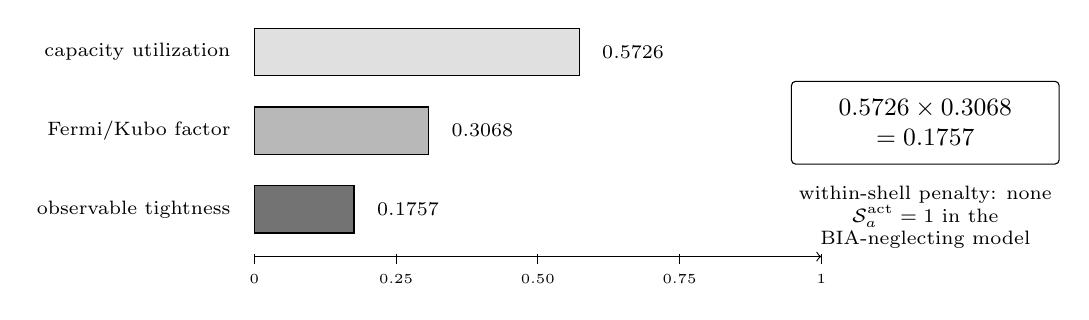
\begin{tikzpicture}[every node/.style={font=\sffamily\small}]
  \def\W{7.2}
  \node[anchor=east,font=\scriptsize] at (0,2.45) {capacity utilization};
  \node[anchor=east,font=\scriptsize] at (0,1.45) {Fermi/Kubo factor};
  \node[anchor=east,font=\scriptsize] at (0,0.45) {observable tightness};
  \draw[fill=black!12,draw=black] (0.18,2.15) rectangle ({0.18+\W*0.57262},2.75);
  \draw[fill=black!28,draw=black] (0.18,1.15) rectangle ({0.18+\W*0.30684},1.75);
  \draw[fill=black!55,draw=black] (0.18,0.15) rectangle ({0.18+\W*0.17570},0.75);
  \node[anchor=west,font=\bfseries\scriptsize] at ({0.35+\W*0.57262},2.45) {$0.5726$};
  \node[anchor=west,font=\bfseries\scriptsize] at ({0.35+\W*0.30684},1.45) {$0.3068$};
  \node[anchor=west,font=\bfseries\scriptsize] at ({0.35+\W*0.17570},0.45) {$0.1757$};
  \draw[->] (0.18,-0.15) -- ({0.18+\W},-0.15);
  \foreach \x/\lab in {0/0,0.25/0.25,0.5/0.50,0.75/0.75,1/1} {
    \draw ({0.18+\W*\x},-0.12) -- ({0.18+\W*\x},-0.24);
    \node[font=\tiny] at ({0.18+\W*\x},-0.43) {\lab};
  }
  \node[draw,rounded corners=1.5pt,align=center,minimum width=3.4cm,minimum height=1.05cm] at (8.70,1.55)
    {$0.5726\times0.3068$\\$=0.1757$};
  \node[align=center,font=\scriptsize] at (8.70,0.35) {within-shell penalty: none\\$\mathcal S_a^{\rm act}=1$ in the\\BIA-neglecting model};
\end{tikzpicture}}
\caption{Production decomposition of the broad-window active-population tightness in the BIA-neglecting second-order eight-band HgCdTe validation. The observed $0.1757$ tightness is explained by shell-to-global capacity utilization and the independent Fermi/Kubo factor; the contributing exact-shell blocks have no additional singular-concentration penalty in this model.}
\label{fig:hgcdte}
\end{figure}%
}

\newcommand{\RevFigRecycling}{%
\begin{figure}[t]
\centering
\resizebox{\columnwidth}{!}{%
\begin{tikzpicture}[>=Latex, every node/.style={font=\sffamily\small}]
  \node[font=\bfseries\small] at (2.55,3.30) {(a) final-sink counting};
  \node[draw,minimum width=1.0cm,minimum height=0.75cm] (A1) at (0.65,1.85) {A};
  \node[draw,minimum width=1.0cm,minimum height=0.75cm] (B1) at (4.45,1.85) {B};
  \draw[->,line width=0.8pt] (A1) -- node[above,font=\scriptsize] {recycle} (B1);
  \node[font=\scriptsize,align=center] at (0.65,0.65) {source terminal\\$H_A^{\rm end}=0$};
  \node[font=\scriptsize,align=center] at (4.45,0.65) {final sink\\$H_B^{\rm end}\ne0$};
  \draw[densely dashed] (A1.south) -- (0.65,1.05);
  \draw[->] (B1.south) -- (4.45,1.05);

  \node[font=\bfseries\small] at (8.30,3.30) {(b) finite-transit Ramo readout};
  \node[draw,minimum width=1.0cm,minimum height=0.75cm] (A2) at (6.30,1.85) {A};
  \node[draw,minimum width=1.0cm,minimum height=0.75cm] (B2) at (10.30,1.85) {B};
  \draw[->,line width=0.8pt] (A2) -- node[above,font=\scriptsize] {recycle / transit} (B2);
  \draw[->] (6.05,0.25) -- (9.25,0.25) node[right,font=\scriptsize] {$t$};
  \draw[->] (6.30,-0.55) -- (6.30,1.05) node[above,font=\scriptsize] {$i_A$};
  \draw[line width=0.85pt]
    plot[smooth] coordinates {(6.30,0.25) (6.65,0.82) (7.05,0.48) (7.45,-0.28) (7.90,-0.05) (8.35,0.25)};
  \node[font=\scriptsize,align=center] at (9.55,0.15) {$\int i_A dt=0$\\but $H_A(\omega\ne0)$ can survive};
  \node[font=\scriptsize,align=center] at (8.25,-0.70) {source-channel endpoint null is lifted at finite frequency};
\end{tikzpicture}}
\caption{Readout-dependent observability of one conservative A-to-B recycling lineage. Final-sink counting assigns the event only to the ultimate sink and can make the source-channel cross contribution identically zero. Finite-transit Shockley--Ramo current can give the internally recombined source segment finite-frequency support even though its integrated induced charge is zero.}
\label{fig:recycling}
\end{figure}%
}
